
\documentclass[UTF8,zihao=5,fontset=fandol]{ctexart}
\usepackage[paperwidth=420mm,paperheight=297mm,margin=0mm]{geometry}
\usepackage{amsmath,amssymb,array,tabularx,graphicx,xcolor,tikz}
\usetikzlibrary{calc,arrows.meta,decorations.pathreplacing}
\definecolor{answerred}{RGB}{180,24,28}
\pagestyle{empty}
\setlength{\parindent}{0pt}
\setlength{\parskip}{0pt}
\setlength{\jot}{0pt}
\setlength{\tabcolsep}{2pt}
\renewcommand{\arraystretch}{1.04}
\newif\ifanswers
\newcommand{\F}[2][2em]{（\makebox[#1][c]{\ifanswers{\color{answerred}#2}\fi}）}
\newcommand{\N}[1]{\textcircled{\scriptsize #1}}
\newcommand{\ans}[1]{{\color{answerred}#1}}
\newcommand{\Q}[2]{\hangindent=1.3em\hangafter=1 #1.\,#2}
\newcommand{\Opt}[4]{\begin{tabularx}{\linewidth}{@{}XXXX@{}}A.\,#1&B.\,#2&C.\,#3&D.\,#4\end{tabularx}}
% Reconstructed from the supplied mathematics test photographs.
% Requires tikz and the arrows.meta library.  No font definitions.
% Orthographic voxel projection: x right, y rear, z up.
% All internal faces are removed. Exterior faces are painter-sorted by
% exact overlap/depth comparisons, so occluded cube edges are not exposed.
\newcommand{\LocationMap}{%
\begin{tikzpicture}[x=8.3mm,y=8.3mm,line cap=round,line join=round,font=\small]
  \draw[step=1,black!65,line width=.32pt] (0,0) grid (5,4);
  \draw[-{Latex[length=1.45mm,width=1.1mm]},line width=.55pt] (0,0) -- (5.35,0);
  \draw[-{Latex[length=1.45mm,width=1.1mm]},line width=.55pt] (0,0) -- (0,4.3);
  \foreach \xx in {0,1,2,3,4,5}
    \node[below=2pt,font=\scriptsize] at (\xx,0) {\xx};
  \foreach \yy in {1,2,3,4}
    \node[left=2pt,font=\scriptsize] at (0,\yy) {\yy};
  \draw[line width=.8pt] (0,0) -- (3,3)
    node[pos=.5,sloped,above=2.5pt,fill=white,inner sep=.8pt,font=\scriptsize] {200米};
  \draw[line width=.4pt] (0,.75) arc[start angle=90,end angle=45,radius=.75];
  \node[fill=white,inner sep=.4pt,font=\scriptsize] at (.32,.88) {$45^\circ$};
  \fill (0,0) circle (1.3pt);
  \node[anchor=east,inner sep=0pt] at (-.25,-.29) {学校};
  \fill (2,3) circle (1.3pt);
  \node[above left=2pt,inner sep=0pt] at (2,3) {书店};
  \fill (3,3) circle (1.3pt);
  \node[above right=2pt,inner sep=0pt] at (3,3) {商店};
  \fill (3,2) circle (1.3pt);
  \node[below right=2pt,inner sep=0pt] at (3,2) {公园};
  \draw[-{Latex[length=1.6mm,width=1.1mm]},line width=.65pt]
    (5.65,3.15) -- (5.65,4.2) node[above=2pt,inner sep=0pt] {北};
\end{tikzpicture}%
}

\newcommand{\SolidChoices}{%
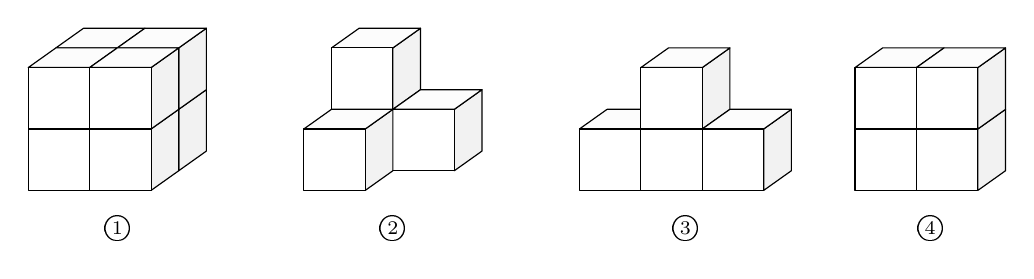
\begin{tikzpicture}[x=7.8mm,y=7.8mm,line cap=round,line join=round,line width=.42pt]

  \begin{scope}[xshift=0mm]
  \path[draw=black,fill=black!1] (0.45,2.32) -- (1.45,2.32) -- (1.9,2.64) -- (0.9,2.64) -- cycle;
  \path[draw=black,fill=black!5] (2.45,0.32) -- (2.9,0.64) -- (2.9,1.64) -- (2.45,1.32) -- cycle;
  \path[draw=black,fill=black!5] (2.45,1.32) -- (2.9,1.64) -- (2.9,2.64) -- (2.45,2.32) -- cycle;
  \path[draw=black,fill=black!1] (1.45,2.32) -- (2.45,2.32) -- (2.9,2.64) -- (1.9,2.64) -- cycle;
  \path[draw=black,fill=black!1] (0,2) -- (1,2) -- (1.45,2.32) -- (0.45,2.32) -- cycle;
  \path[draw=black,fill=black!5] (2,0) -- (2.45,0.32) -- (2.45,1.32) -- (2,1) -- cycle;
  \path[draw=black,fill=black!5] (2,1) -- (2.45,1.32) -- (2.45,2.32) -- (2,2) -- cycle;
  \path[draw=black,fill=black!1] (1,2) -- (2,2) -- (2.45,2.32) -- (1.45,2.32) -- cycle;
  \path[draw=black,fill=white] (0,0) -- (1,0) -- (1,1) -- (0,1) -- cycle;
  \path[draw=black,fill=white] (0,1) -- (1,1) -- (1,2) -- (0,2) -- cycle;
  \path[draw=black,fill=white] (1,0) -- (2,0) -- (2,1) -- (1,1) -- cycle;
  \path[draw=black,fill=white] (1,1) -- (2,1) -- (2,2) -- (1,2) -- cycle;
  \node[below=0pt,font=\small] at (1.45,-.35) {\textcircled{\scriptsize 1}};
  \end{scope}
  \begin{scope}[xshift=35mm]
  \path[draw=black,fill=black!5] (1.45,1.32) -- (1.9,1.64) -- (1.9,2.64) -- (1.45,2.32) -- cycle;
  \path[draw=black,fill=black!1] (0.45,2.32) -- (1.45,2.32) -- (1.9,2.64) -- (0.9,2.64) -- cycle;
  \path[draw=black,fill=black!5] (2.45,0.32) -- (2.9,0.64) -- (2.9,1.64) -- (2.45,1.32) -- cycle;
  \path[draw=black,fill=black!1] (1.45,1.32) -- (2.45,1.32) -- (2.9,1.64) -- (1.9,1.64) -- cycle;
  \path[draw=black,fill=white] (0.45,1.32) -- (1.45,1.32) -- (1.45,2.32) -- (0.45,2.32) -- cycle;
  \path[draw=black,fill=white] (1.45,0.32) -- (2.45,0.32) -- (2.45,1.32) -- (1.45,1.32) -- cycle;
  \path[draw=black,fill=black!5] (1,0) -- (1.45,0.32) -- (1.45,1.32) -- (1,1) -- cycle;
  \path[draw=black,fill=black!1] (0,1) -- (1,1) -- (1.45,1.32) -- (0.45,1.32) -- cycle;
  \path[draw=black,fill=white] (0,0) -- (1,0) -- (1,1) -- (0,1) -- cycle;
  \node[below=0pt,font=\small] at (1.45,-.35) {\textcircled{\scriptsize 2}};
  \end{scope}
  \begin{scope}[xshift=70mm]
  \path[draw=black,fill=black!1] (0,1) -- (1,1) -- (1.45,1.32) -- (0.45,1.32) -- cycle;
  \path[draw=black,fill=black!5] (2,1) -- (2.45,1.32) -- (2.45,2.32) -- (2,2) -- cycle;
  \path[draw=black,fill=black!1] (1,2) -- (2,2) -- (2.45,2.32) -- (1.45,2.32) -- cycle;
  \path[draw=black,fill=black!5] (3,0) -- (3.45,0.32) -- (3.45,1.32) -- (3,1) -- cycle;
  \path[draw=black,fill=black!1] (2,1) -- (3,1) -- (3.45,1.32) -- (2.45,1.32) -- cycle;
  \path[draw=black,fill=white] (0,0) -- (1,0) -- (1,1) -- (0,1) -- cycle;
  \path[draw=black,fill=white] (1,0) -- (2,0) -- (2,1) -- (1,1) -- cycle;
  \path[draw=black,fill=white] (1,1) -- (2,1) -- (2,2) -- (1,2) -- cycle;
  \path[draw=black,fill=white] (2,0) -- (3,0) -- (3,1) -- (2,1) -- cycle;
  \node[below=0pt,font=\small] at (1.725,-.35) {\textcircled{\scriptsize 3}};
  \end{scope}
  \begin{scope}[xshift=105mm]
  \path[draw=black,fill=black!1] (0,2) -- (1,2) -- (1.45,2.32) -- (0.45,2.32) -- cycle;
  \path[draw=black,fill=black!5] (2,0) -- (2.45,0.32) -- (2.45,1.32) -- (2,1) -- cycle;
  \path[draw=black,fill=black!5] (2,1) -- (2.45,1.32) -- (2.45,2.32) -- (2,2) -- cycle;
  \path[draw=black,fill=black!1] (1,2) -- (2,2) -- (2.45,2.32) -- (1.45,2.32) -- cycle;
  \path[draw=black,fill=white] (0,0) -- (1,0) -- (1,1) -- (0,1) -- cycle;
  \path[draw=black,fill=white] (0,1) -- (1,1) -- (1,2) -- (0,2) -- cycle;
  \path[draw=black,fill=white] (1,0) -- (2,0) -- (2,1) -- (1,1) -- cycle;
  \path[draw=black,fill=white] (1,1) -- (2,1) -- (2,2) -- (1,2) -- cycle;
  \node[below=0pt,font=\small] at (1.225,-.35) {\textcircled{\scriptsize 4}};
  \end{scope}
\end{tikzpicture}%
}

\newcommand{\StepPyramid}{%
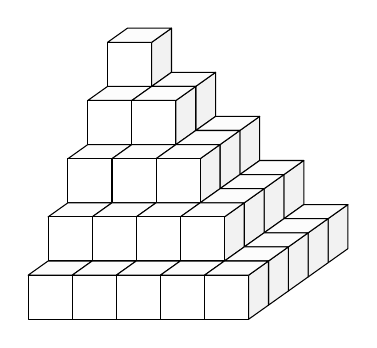
\begin{tikzpicture}[x=5.6mm,y=5.6mm,line cap=round,line join=round,line width=.38pt]
  \path[draw=black,fill=black!5] (2.8,5.28) -- (3.25,5.6) -- (3.25,6.6) -- (2.8,6.28) -- cycle;
  \path[draw=black,fill=black!1] (1.8,6.28) -- (2.8,6.28) -- (3.25,6.6) -- (2.25,6.6) -- cycle;
  \path[draw=black,fill=black!5] (3.8,4.28) -- (4.25,4.6) -- (4.25,5.6) -- (3.8,5.28) -- cycle;
  \path[draw=black,fill=black!1] (2.8,5.28) -- (3.8,5.28) -- (4.25,5.6) -- (3.25,5.6) -- cycle;
  \path[draw=black,fill=black!5] (4.8,3.28) -- (5.25,3.6) -- (5.25,4.6) -- (4.8,4.28) -- cycle;
  \path[draw=black,fill=black!1] (3.8,4.28) -- (4.8,4.28) -- (5.25,4.6) -- (4.25,4.6) -- cycle;
  \path[draw=black,fill=black!5] (5.8,2.28) -- (6.25,2.6) -- (6.25,3.6) -- (5.8,3.28) -- cycle;
  \path[draw=black,fill=black!1] (4.8,3.28) -- (5.8,3.28) -- (6.25,3.6) -- (5.25,3.6) -- cycle;
  \path[draw=black,fill=black!5] (6.8,1.28) -- (7.25,1.6) -- (7.25,2.6) -- (6.8,2.28) -- cycle;
  \path[draw=black,fill=black!1] (5.8,2.28) -- (6.8,2.28) -- (7.25,2.6) -- (6.25,2.6) -- cycle;
  \path[draw=black,fill=white] (1.8,5.28) -- (2.8,5.28) -- (2.8,6.28) -- (1.8,6.28) -- cycle;
  \path[draw=black,fill=black!1] (1.35,4.96) -- (2.35,4.96) -- (2.8,5.28) -- (1.8,5.28) -- cycle;
  \path[draw=black,fill=black!5] (3.35,3.96) -- (3.8,4.28) -- (3.8,5.28) -- (3.35,4.96) -- cycle;
  \path[draw=black,fill=black!1] (2.35,4.96) -- (3.35,4.96) -- (3.8,5.28) -- (2.8,5.28) -- cycle;
  \path[draw=black,fill=black!5] (4.35,2.96) -- (4.8,3.28) -- (4.8,4.28) -- (4.35,3.96) -- cycle;
  \path[draw=black,fill=black!1] (3.35,3.96) -- (4.35,3.96) -- (4.8,4.28) -- (3.8,4.28) -- cycle;
  \path[draw=black,fill=black!5] (5.35,1.96) -- (5.8,2.28) -- (5.8,3.28) -- (5.35,2.96) -- cycle;
  \path[draw=black,fill=black!1] (4.35,2.96) -- (5.35,2.96) -- (5.8,3.28) -- (4.8,3.28) -- cycle;
  \path[draw=black,fill=black!5] (6.35,0.96) -- (6.8,1.28) -- (6.8,2.28) -- (6.35,1.96) -- cycle;
  \path[draw=black,fill=black!1] (5.35,1.96) -- (6.35,1.96) -- (6.8,2.28) -- (5.8,2.28) -- cycle;
  \path[draw=black,fill=white] (1.35,3.96) -- (2.35,3.96) -- (2.35,4.96) -- (1.35,4.96) -- cycle;
  \path[draw=black,fill=white] (2.35,3.96) -- (3.35,3.96) -- (3.35,4.96) -- (2.35,4.96) -- cycle;
  \path[draw=black,fill=black!1] (0.9,3.64) -- (1.9,3.64) -- (2.35,3.96) -- (1.35,3.96) -- cycle;
  \path[draw=black,fill=black!1] (1.9,3.64) -- (2.9,3.64) -- (3.35,3.96) -- (2.35,3.96) -- cycle;
  \path[draw=black,fill=black!5] (3.9,2.64) -- (4.35,2.96) -- (4.35,3.96) -- (3.9,3.64) -- cycle;
  \path[draw=black,fill=black!1] (2.9,3.64) -- (3.9,3.64) -- (4.35,3.96) -- (3.35,3.96) -- cycle;
  \path[draw=black,fill=black!5] (4.9,1.64) -- (5.35,1.96) -- (5.35,2.96) -- (4.9,2.64) -- cycle;
  \path[draw=black,fill=black!1] (3.9,2.64) -- (4.9,2.64) -- (5.35,2.96) -- (4.35,2.96) -- cycle;
  \path[draw=black,fill=black!5] (5.9,0.64) -- (6.35,0.96) -- (6.35,1.96) -- (5.9,1.64) -- cycle;
  \path[draw=black,fill=black!1] (4.9,1.64) -- (5.9,1.64) -- (6.35,1.96) -- (5.35,1.96) -- cycle;
  \path[draw=black,fill=white] (0.9,2.64) -- (1.9,2.64) -- (1.9,3.64) -- (0.9,3.64) -- cycle;
  \path[draw=black,fill=white] (1.9,2.64) -- (2.9,2.64) -- (2.9,3.64) -- (1.9,3.64) -- cycle;
  \path[draw=black,fill=white] (2.9,2.64) -- (3.9,2.64) -- (3.9,3.64) -- (2.9,3.64) -- cycle;
  \path[draw=black,fill=black!1] (0.45,2.32) -- (1.45,2.32) -- (1.9,2.64) -- (0.9,2.64) -- cycle;
  \path[draw=black,fill=black!1] (1.45,2.32) -- (2.45,2.32) -- (2.9,2.64) -- (1.9,2.64) -- cycle;
  \path[draw=black,fill=black!1] (2.45,2.32) -- (3.45,2.32) -- (3.9,2.64) -- (2.9,2.64) -- cycle;
  \path[draw=black,fill=black!5] (4.45,1.32) -- (4.9,1.64) -- (4.9,2.64) -- (4.45,2.32) -- cycle;
  \path[draw=black,fill=black!1] (3.45,2.32) -- (4.45,2.32) -- (4.9,2.64) -- (3.9,2.64) -- cycle;
  \path[draw=black,fill=black!5] (5.45,0.32) -- (5.9,0.64) -- (5.9,1.64) -- (5.45,1.32) -- cycle;
  \path[draw=black,fill=black!1] (4.45,1.32) -- (5.45,1.32) -- (5.9,1.64) -- (4.9,1.64) -- cycle;
  \path[draw=black,fill=white] (0.45,1.32) -- (1.45,1.32) -- (1.45,2.32) -- (0.45,2.32) -- cycle;
  \path[draw=black,fill=white] (1.45,1.32) -- (2.45,1.32) -- (2.45,2.32) -- (1.45,2.32) -- cycle;
  \path[draw=black,fill=white] (2.45,1.32) -- (3.45,1.32) -- (3.45,2.32) -- (2.45,2.32) -- cycle;
  \path[draw=black,fill=white] (3.45,1.32) -- (4.45,1.32) -- (4.45,2.32) -- (3.45,2.32) -- cycle;
  \path[draw=black,fill=black!1] (0,1) -- (1,1) -- (1.45,1.32) -- (0.45,1.32) -- cycle;
  \path[draw=black,fill=black!1] (1,1) -- (2,1) -- (2.45,1.32) -- (1.45,1.32) -- cycle;
  \path[draw=black,fill=black!1] (2,1) -- (3,1) -- (3.45,1.32) -- (2.45,1.32) -- cycle;
  \path[draw=black,fill=black!1] (3,1) -- (4,1) -- (4.45,1.32) -- (3.45,1.32) -- cycle;
  \path[draw=black,fill=black!5] (5,0) -- (5.45,0.32) -- (5.45,1.32) -- (5,1) -- cycle;
  \path[draw=black,fill=black!1] (4,1) -- (5,1) -- (5.45,1.32) -- (4.45,1.32) -- cycle;
  \path[draw=black,fill=white] (0,0) -- (1,0) -- (1,1) -- (0,1) -- cycle;
  \path[draw=black,fill=white] (1,0) -- (2,0) -- (2,1) -- (1,1) -- cycle;
  \path[draw=black,fill=white] (2,0) -- (3,0) -- (3,1) -- (2,1) -- cycle;
  \path[draw=black,fill=white] (3,0) -- (4,0) -- (4,1) -- (3,1) -- cycle;
  \path[draw=black,fill=white] (4,0) -- (5,0) -- (5,1) -- (4,1) -- cycle;
\end{tikzpicture}%
}

\newcommand{\DistanceDiagram}{%
\begin{tikzpicture}[x=1cm,y=1cm,line width=.45pt,font=\fontsize{9}{11}\selectfont]
\draw (0,0)--(4,0);
\foreach \x in {0,1,2,3,4}{\draw (\x,-.08)--(\x,.08);}
\draw[decorate,decoration={brace,amplitude=3pt}] (0,.18)--(4,.18) node[midway,above=4pt]{48千米};
\draw[decorate,decoration={brace,mirror,amplitude=3pt}] (0,-.18)--(3,-.18) node[midway,below=4pt]{？千米};
\end{tikzpicture}}
\newcommand{\MelonDiagram}{%
\begin{tikzpicture}[x=.65cm,y=1cm,line width=.45pt,font=\fontsize{9}{11}\selectfont]
\node[left] at (-.08,0){西瓜：};
\node[left] at (-.08,-.55){甜瓜：};
\draw (0,0)--(7,0);
\foreach \x in {0,1,2,3,4,5,6,7}{\draw (\x,-.07)--(\x,.07);}
\draw (0,-.55)--(5,-.55);
\foreach \x in {0,1,2,3,4,5}{\draw (\x,-.62)--(\x,-.48);}
\draw[densely dashed,line width=.3pt] (5,-.11)--(5,-.44);
\draw[decorate,decoration={brace,amplitude=3pt}] (0,.18)--(7,.18) node[midway,above=4pt]{$a$千克};
\draw[decorate,decoration={brace,mirror,amplitude=3pt}] (0,-.73)--(5,-.73) node[midway,below=4pt]{350千克};
\end{tikzpicture}}
\newcommand{\PrizeDiagram}{%
\begin{tikzpicture}[x=.75cm,y=.49cm,line width=.4pt,font=\fontsize{8}{10}\selectfont]
\node[left] at (-.15,0){三等奖};
\node[left] at (-.15,-1){二等奖};
\node[left] at (-.15,-2){一等奖};
\draw (0,0)--(4,0);
\foreach \x in {0,1,2,3,4}{\draw (\x,-.12)--(\x,.12);}
\draw (0,-1)--(3,-1);
\foreach \x in {0,1,2,3}{\draw (\x,-1.12)--(\x,-.88);}
\draw (0,-2)--(2,-2);
\foreach \x in {0,1,2}{\draw (\x,-2.12)--(\x,-1.88);}
\node[right] at (4.08,0){120人};
\node[right] at (2.08,-2){？人};
\end{tikzpicture}}
\newcommand{\InfoTable}{%
\begin{tabularx}{\linewidth}{|>{\raggedright\arraybackslash}X|}
\hline
\N{1}\ 四年级有204人。\\[2pt]\hline
\N{2}\ 四年级喜欢打篮球的人数比总人数的 $\frac4{17}$ 多5人。\\[2pt]\hline
\N{3}\ 四年级学生人数是五年级人数的 $\frac{34}{31}$。\\[2pt]\hline
\N{4}\ 五年级女生占年级总人数的 $\frac{14}{31}$。\\[2pt]\hline
\end{tabularx}}

\answerstrue
\begin{document}
\begin{tikzpicture}[remember picture,overlay]
\begin{scope}[shift={(current page.north west)},x=1mm,y=-1mm]
\draw[line width=.28pt] (220,36)--(220,262);
\draw[line width=.28pt,densely dashed] (47,64)--(47,244);
\node[anchor=north west,inner sep=0pt,outer sep=0pt] (b0) at (76,38) {\begin{minipage}[t]{112mm}\fontsize{14}{18}\selectfont\setlength{\parskip}{0pt}\raggedright \centering\heiti 五年级数学小测\end{minipage}};
\path let \p1=(b0.north),\p2=(b0.south) in \pgfextra{\pgfmathsetmacro{\bh}{(\y1-\y2)/1mm}\typeout{BLOCKH:b0:\bh}};
\node[anchor=north west,inner sep=0pt,outer sep=0pt] (b1) at (77,48) {\begin{minipage}[t]{110mm}\fontsize{8.5}{11}\selectfont\setlength{\parskip}{0pt}\raggedright \centering （满分：100分；建议用时：90分钟）\end{minipage}};
\path let \p1=(b1.north),\p2=(b1.south) in \pgfextra{\pgfmathsetmacro{\bh}{(\y1-\y2)/1mm}\typeout{BLOCKH:b1:\bh}};
\node[anchor=north west,inner sep=0pt,outer sep=0pt] (b2) at (164,54) {\begin{minipage}[t]{32mm}\fontsize{8.5}{11}\selectfont\setlength{\parskip}{0pt}\raggedright \begin{tabular}{|p{10mm}|p{16mm}|}\hline 等\quad 级&\\[3pt]\hline\end{tabular}\end{minipage}};
\path let \p1=(b2.north),\p2=(b2.south) in \pgfextra{\pgfmathsetmacro{\bh}{(\y1-\y2)/1mm}\typeout{BLOCKH:b2:\bh}};
\node[anchor=north west,inner sep=0pt,outer sep=0pt] (b3) at (55,66) {\begin{minipage}[t]{143mm}\fontsize{9.6}{13}\selectfont\setlength{\parskip}{0pt}\raggedright \heiti 一、认真思考，正确填写。（32分）\end{minipage}};
\path let \p1=(b3.north),\p2=(b3.south) in \pgfextra{\pgfmathsetmacro{\bh}{(\y1-\y2)/1mm}\typeout{BLOCKH:b3:\bh}};
\node[anchor=north west,inner sep=0pt,outer sep=0pt] (b4) at (55,74) {\begin{minipage}[t]{143mm}\fontsize{8.9}{14.5}\selectfont\setlength{\parskip}{0pt}\raggedright \Q{1}{计算 $\frac34+\frac15$ 时，由于\F[4em]{分数单位}不同，所以要先通分。$\frac34$ 是\F[1.6em]{15}个 $\frac1{20}$，$\frac15$ 是\F[1.5em]{4}个 $\frac1{20}$，它们的和是\F[1.6em]{19}个 $\frac1{20}$。}\end{minipage}};
\path let \p1=(b4.north),\p2=(b4.south) in \pgfextra{\pgfmathsetmacro{\bh}{(\y1-\y2)/1mm}\typeout{BLOCKH:b4:\bh}};
\node[anchor=north west,inner sep=0pt,outer sep=0pt] (b5) at (55,94) {\begin{minipage}[t]{143mm}\fontsize{9.1}{13.4}\selectfont\setlength{\parskip}{0pt}\raggedright \Q{2}{一桶油重8千克，$\frac25$ 桶油重\F[2.1em]{$\frac{16}{5}$}千克。}\end{minipage}};
\path let \p1=(b5.north),\p2=(b5.south) in \pgfextra{\pgfmathsetmacro{\bh}{(\y1-\y2)/1mm}\typeout{BLOCKH:b5:\bh}};
\node[anchor=north west,inner sep=0pt,outer sep=0pt] (b6) at (55,105) {\begin{minipage}[t]{143mm}\fontsize{9.1}{13.4}\selectfont\setlength{\parskip}{0pt}\raggedright \Q{3}{$\frac35$ 升$=$\F[2.6em]{600}毫升\qquad $18.9$升$=$\F[2.4em]{18.9}立方分米$=$\F[2.8em]{18900}立方厘米}\end{minipage}};
\path let \p1=(b6.north),\p2=(b6.south) in \pgfextra{\pgfmathsetmacro{\bh}{(\y1-\y2)/1mm}\typeout{BLOCKH:b6:\bh}};
\node[anchor=north west,inner sep=0pt,outer sep=0pt] (b7) at (59,116) {\begin{minipage}[t]{139mm}\fontsize{9.1}{13.4}\selectfont\setlength{\parskip}{0pt}\raggedright $\frac34$ 分$=$\F[2.6em]{45}秒\qquad\quad $3.06$立方米$=$\F[1.6em]{3}立方米\F[1.8em]{60}立方分米。\end{minipage}};
\path let \p1=(b7.north),\p2=(b7.south) in \pgfextra{\pgfmathsetmacro{\bh}{(\y1-\y2)/1mm}\typeout{BLOCKH:b7:\bh}};
\node[anchor=north west,inner sep=0pt,outer sep=0pt] (b8) at (55,126) {\begin{minipage}[t]{143mm}\fontsize{8.9}{13.3}\selectfont\setlength{\parskip}{0pt}\raggedright \Q{4}{用一根48米的铁丝焊接成一个正方体的框架，这个正方体框架的棱长是\F[1.4em]{4}米；如果在这个框架的表面贴上彩纸，至少需要\F[1.6em]{96}平方米的彩纸。}\end{minipage}};
\path let \p1=(b8.north),\p2=(b8.south) in \pgfextra{\pgfmathsetmacro{\bh}{(\y1-\y2)/1mm}\typeout{BLOCKH:b8:\bh}};
\node[anchor=north west,inner sep=0pt,outer sep=0pt] (b9) at (55,143) {\begin{minipage}[t]{143mm}\fontsize{8.9}{12}\selectfont\setlength{\parskip}{0pt}\raggedright \Q{5}{$\dfrac58\times$\F[1.9em]{$\frac85$}$=$\F[2.2em]{$\frac{16}{21}$}$+\dfrac5{21}=0.25\times$\F[1.5em]{4}$=1\dfrac34\times$\F[1.9em]{$\frac47$}$=1$。}\end{minipage}};
\path let \p1=(b9.north),\p2=(b9.south) in \pgfextra{\pgfmathsetmacro{\bh}{(\y1-\y2)/1mm}\typeout{BLOCKH:b9:\bh}};
\node[anchor=north west,inner sep=0pt,outer sep=0pt] (b10) at (55,154) {\begin{minipage}[t]{143mm}\fontsize{9.1}{13.4}\selectfont\setlength{\parskip}{0pt}\raggedright \Q{6}{在 $\bigcirc$ 里填上“$>$”“$<$”或“$=$”。}\end{minipage}};
\path let \p1=(b10.north),\p2=(b10.south) in \pgfextra{\pgfmathsetmacro{\bh}{(\y1-\y2)/1mm}\typeout{BLOCKH:b10:\bh}};
\node[anchor=north west,inner sep=0pt,outer sep=0pt] (b11) at (60,162) {\begin{minipage}[t]{28mm}\fontsize{8.8}{12}\selectfont\setlength{\parskip}{0pt}\raggedright $\displaystyle \frac5{12}\mathbin{\makebox[1em][c]{\ifanswers\ans{$<$}\else$\bigcirc$\fi}}\frac{11}{18}$\end{minipage}};
\path let \p1=(b11.north),\p2=(b11.south) in \pgfextra{\pgfmathsetmacro{\bh}{(\y1-\y2)/1mm}\typeout{BLOCKH:b11:\bh}};
\node[anchor=north west,inner sep=0pt,outer sep=0pt] (b12) at (90,162) {\begin{minipage}[t]{35mm}\fontsize{8.8}{12}\selectfont\setlength{\parskip}{0pt}\raggedright $\displaystyle \frac35\times\frac34\mathbin{\makebox[1em][c]{\ifanswers\ans{$<$}\else$\bigcirc$\fi}}\frac35$\end{minipage}};
\path let \p1=(b12.north),\p2=(b12.south) in \pgfextra{\pgfmathsetmacro{\bh}{(\y1-\y2)/1mm}\typeout{BLOCKH:b12:\bh}};
\node[anchor=north west,inner sep=0pt,outer sep=0pt] (b13) at (126,162) {\begin{minipage}[t]{35mm}\fontsize{8.8}{12}\selectfont\setlength{\parskip}{0pt}\raggedright $\displaystyle \frac9{23}\div\frac78\mathbin{\makebox[1em][c]{\ifanswers\ans{$>$}\else$\bigcirc$\fi}}\frac9{23}$\end{minipage}};
\path let \p1=(b13.north),\p2=(b13.south) in \pgfextra{\pgfmathsetmacro{\bh}{(\y1-\y2)/1mm}\typeout{BLOCKH:b13:\bh}};
\node[anchor=north west,inner sep=0pt,outer sep=0pt] (b14) at (162,162) {\begin{minipage}[t]{36mm}\fontsize{8.8}{12}\selectfont\setlength{\parskip}{0pt}\raggedright $\displaystyle \frac16+\frac34\mathbin{\makebox[1em][c]{\ifanswers\ans{$>$}\else$\bigcirc$\fi}}\frac16\times\frac34$\end{minipage}};
\path let \p1=(b14.north),\p2=(b14.south) in \pgfextra{\pgfmathsetmacro{\bh}{(\y1-\y2)/1mm}\typeout{BLOCKH:b14:\bh}};
\node[anchor=north west,inner sep=0pt,outer sep=0pt] (b15) at (55,173) {\begin{minipage}[t]{143mm}\fontsize{9.1}{13.4}\selectfont\setlength{\parskip}{0pt}\raggedright \Q{7}{在括号里填上合适的单位名称。}\end{minipage}};
\path let \p1=(b15.north),\p2=(b15.south) in \pgfextra{\pgfmathsetmacro{\bh}{(\y1-\y2)/1mm}\typeout{BLOCKH:b15:\bh}};
\node[anchor=north west,inner sep=0pt,outer sep=0pt] (b16) at (59,181) {\begin{minipage}[t]{67mm}\fontsize{8.5}{11}\selectfont\setlength{\parskip}{0pt}\raggedright 一个西瓜的体积约是8\F[4em]{立方分米}。\end{minipage}};
\path let \p1=(b16.north),\p2=(b16.south) in \pgfextra{\pgfmathsetmacro{\bh}{(\y1-\y2)/1mm}\typeout{BLOCKH:b16:\bh}};
\node[anchor=north west,inner sep=0pt,outer sep=0pt] (b17) at (128,181) {\begin{minipage}[t]{70mm}\fontsize{8.5}{11}\selectfont\setlength{\parskip}{0pt}\raggedright 学校操场沙坑的容积约是6\F[3em]{立方米}。\end{minipage}};
\path let \p1=(b17.north),\p2=(b17.south) in \pgfextra{\pgfmathsetmacro{\bh}{(\y1-\y2)/1mm}\typeout{BLOCKH:b17:\bh}};
\node[anchor=north west,inner sep=0pt,outer sep=0pt] (b18) at (59,189) {\begin{minipage}[t]{67mm}\fontsize{8.5}{11}\selectfont\setlength{\parskip}{0pt}\raggedright 一盒牛奶有500\F[3em]{毫升}。\end{minipage}};
\path let \p1=(b18.north),\p2=(b18.south) in \pgfextra{\pgfmathsetmacro{\bh}{(\y1-\y2)/1mm}\typeout{BLOCKH:b18:\bh}};
\node[anchor=north west,inner sep=0pt,outer sep=0pt] (b19) at (128,189) {\begin{minipage}[t]{70mm}\fontsize{8.5}{11}\selectfont\setlength{\parskip}{0pt}\raggedright 冰箱的容积约是190\F[3em]{升}。\end{minipage}};
\path let \p1=(b19.north),\p2=(b19.south) in \pgfextra{\pgfmathsetmacro{\bh}{(\y1-\y2)/1mm}\typeout{BLOCKH:b19:\bh}};
\node[anchor=north west,inner sep=0pt,outer sep=0pt] (b20) at (55,198) {\begin{minipage}[t]{143mm}\fontsize{8.8}{12}\selectfont\setlength{\parskip}{0pt}\raggedright \Q{8}{学校舞蹈队有女生60人，占总人数的 $\frac34$，舞蹈队总人数有多少人？数量关系式是}\end{minipage}};
\path let \p1=(b20.north),\p2=(b20.south) in \pgfextra{\pgfmathsetmacro{\bh}{(\y1-\y2)/1mm}\typeout{BLOCKH:b20:\bh}};
\node[anchor=north west,inner sep=0pt,outer sep=0pt] (b21) at (58,207) {\begin{minipage}[t]{140mm}\fontsize{9}{12}\selectfont\setlength{\parskip}{0pt}\raggedright \F[8em]{舞蹈队总人数}$\times\dfrac34=$\F[8.5em]{舞蹈队女生人数}。\end{minipage}};
\path let \p1=(b21.north),\p2=(b21.south) in \pgfextra{\pgfmathsetmacro{\bh}{(\y1-\y2)/1mm}\typeout{BLOCKH:b21:\bh}};
\node[anchor=north west,inner sep=0pt,outer sep=0pt] (b22) at (55,217) {\begin{minipage}[t]{143mm}\fontsize{8.5}{12}\selectfont\setlength{\parskip}{0pt}\raggedright \Q{9}{一个蓄水池，长10米、宽4米、深2米，蓄水池占地面积是\F[4.4em]{40平方米}；在蓄水池的底部和四周都抹上水泥，抹水泥的面积是\F[4.4em]{96平方米}；池内最多能容水\F[3.2em]{80000}升。}\end{minipage}};
\path let \p1=(b22.north),\p2=(b22.south) in \pgfextra{\pgfmathsetmacro{\bh}{(\y1-\y2)/1mm}\typeout{BLOCKH:b22:\bh}};
\node[anchor=north west,inner sep=0pt,outer sep=0pt] (b23) at (55,232) {\begin{minipage}[t]{106mm}\fontsize{8.7}{13}\selectfont\setlength{\parskip}{0pt}\raggedright \Q{10}{6个棱长1分米的正方体纸盒放在墙角，如右图，体积是\F[1.5em]{6}立方分米，露在外面的面积之和是\F[2.5em]{待核}平方分米。}\end{minipage}};
\path let \p1=(b23.north),\p2=(b23.south) in \pgfextra{\pgfmathsetmacro{\bh}{(\y1-\y2)/1mm}\typeout{BLOCKH:b23:\bh}};
\node[anchor=north west,inner sep=0pt,outer sep=0pt] (b24) at (165,230) {\begin{minipage}[t]{32mm}\fontsize{8}{10}\selectfont\setlength{\parskip}{0pt}\raggedright 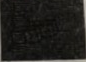
\includegraphics[width=31mm,height=24mm]{原题模糊图.png}\end{minipage}};
\path let \p1=(b24.north),\p2=(b24.south) in \pgfextra{\pgfmathsetmacro{\bh}{(\y1-\y2)/1mm}\typeout{BLOCKH:b24:\bh}};
\node[anchor=north west,inner sep=0pt,outer sep=0pt] (b25) at (55,250) {\begin{minipage}[t]{105mm}\fontsize{8.7}{13}\selectfont\setlength{\parskip}{0pt}\raggedright \Q{11}{水果市场上午卖出水果 $\frac38$ 吨，下午比上午多卖出 $\frac1{12}$ 吨，这一天一共卖出\F[2em]{$\frac56$}吨？}\end{minipage}};
\path let \p1=(b25.north),\p2=(b25.south) in \pgfextra{\pgfmathsetmacro{\bh}{(\y1-\y2)/1mm}\typeout{BLOCKH:b25:\bh}};
\node[anchor=north west,inner sep=0pt,outer sep=0pt] (b26) at (55,271) {\begin{minipage}[t]{143mm}\fontsize{6.6}{8.4}\selectfont\setlength{\parskip}{0pt}\raggedright 第10题右图在原照片中过暗，外露面积待补充清晰图后核定。\end{minipage}};
\path let \p1=(b26.north),\p2=(b26.south) in \pgfextra{\pgfmathsetmacro{\bh}{(\y1-\y2)/1mm}\typeout{BLOCKH:b26:\bh}};
\node[anchor=north west,inner sep=0pt,outer sep=0pt] (b27) at (250,36) {\begin{minipage}[t]{145mm}\fontsize{9}{13.2}\selectfont\setlength{\parskip}{0pt}\raggedright \Q{12}{《庄子》载：“一尺之棰，日取其半，万世不竭”。照此说法，第\F[1.5em]{4}天取的长度\\是 $\frac1{16}$ 尺。}\end{minipage}};
\path let \p1=(b27.north),\p2=(b27.south) in \pgfextra{\pgfmathsetmacro{\bh}{(\y1-\y2)/1mm}\typeout{BLOCKH:b27:\bh}};
\node[anchor=north west,inner sep=0pt,outer sep=0pt] (b28) at (250,56) {\begin{minipage}[t]{145mm}\fontsize{9.1}{12}\selectfont\setlength{\parskip}{0pt}\raggedright {\heiti 二、慎重考虑，合理选择。}\ {\fontsize{7.8}{10}\selectfont （把正确答案的序号填在括号里）}\ （10分）\end{minipage}};
\path let \p1=(b28.north),\p2=(b28.south) in \pgfextra{\pgfmathsetmacro{\bh}{(\y1-\y2)/1mm}\typeout{BLOCKH:b28:\bh}};
\node[anchor=north west,inner sep=0pt,outer sep=0pt] (b29) at (250,65) {\begin{minipage}[t]{103mm}\fontsize{9}{13}\selectfont\setlength{\parskip}{0pt}\raggedright \Q{1}{观察右图，学校在商店的\F[1.5em]{A}45°约200米处，数对（2，3）表示\F[1.5em]{D}的位置。}\end{minipage}};
\path let \p1=(b29.north),\p2=(b29.south) in \pgfextra{\pgfmathsetmacro{\bh}{(\y1-\y2)/1mm}\typeout{BLOCKH:b29:\bh}};
\node[anchor=north west,inner sep=0pt,outer sep=0pt] (b30) at (257,82) {\begin{minipage}[t]{96mm}\fontsize{8.3}{11}\selectfont\setlength{\parskip}{0pt}\raggedright \Opt{南偏西}{北偏东}{公园}{书店}\end{minipage}};
\path let \p1=(b30.north),\p2=(b30.south) in \pgfextra{\pgfmathsetmacro{\bh}{(\y1-\y2)/1mm}\typeout{BLOCKH:b30:\bh}};
\node[anchor=north west,inner sep=0pt,outer sep=0pt] (b31) at (354,65) {\begin{minipage}[t]{39mm}\fontsize{8}{10}\selectfont\setlength{\parskip}{0pt}\raggedright \resizebox{38mm}{!}{\LocationMap}\end{minipage}};
\path let \p1=(b31.north),\p2=(b31.south) in \pgfextra{\pgfmathsetmacro{\bh}{(\y1-\y2)/1mm}\typeout{BLOCKH:b31:\bh}};
\node[anchor=north west,inner sep=0pt,outer sep=0pt] (b32) at (250,88) {\begin{minipage}[t]{103mm}\fontsize{9}{13}\selectfont\setlength{\parskip}{0pt}\raggedright \Q{2}{一个长方体正好可以切成两个棱长是3厘米的正方体，这个长方体的表面积是\F[1.5em]{C}。}\end{minipage}};
\path let \p1=(b32.north),\p2=(b32.south) in \pgfextra{\pgfmathsetmacro{\bh}{(\y1-\y2)/1mm}\typeout{BLOCKH:b32:\bh}};
\node[anchor=north west,inner sep=0pt,outer sep=0pt] (b33) at (250,104) {\begin{minipage}[t]{145mm}\fontsize{8.3}{11}\selectfont\setlength{\parskip}{0pt}\raggedright \Opt{108平方厘米}{54平方厘米}{90平方厘米}{99平方厘米}\end{minipage}};
\path let \p1=(b33.north),\p2=(b33.south) in \pgfextra{\pgfmathsetmacro{\bh}{(\y1-\y2)/1mm}\typeout{BLOCKH:b33:\bh}};
\node[anchor=north west,inner sep=0pt,outer sep=0pt] (b34) at (250,112) {\begin{minipage}[t]{145mm}\fontsize{9}{12.8}\selectfont\setlength{\parskip}{0pt}\raggedright \Q{3}{用一根长80厘米的铁丝正好可以焊成一个高5厘米、宽4厘米、长\F[1.5em]{D}厘米的长方体框架？}\end{minipage}};
\path let \p1=(b34.north),\p2=(b34.south) in \pgfextra{\pgfmathsetmacro{\bh}{(\y1-\y2)/1mm}\typeout{BLOCKH:b34:\bh}};
\node[anchor=north west,inner sep=0pt,outer sep=0pt] (b35) at (280,120) {\begin{minipage}[t]{110mm}\fontsize{8.7}{11}\selectfont\setlength{\parskip}{0pt}\raggedright \Opt{7}{8}{4}{11}\end{minipage}};
\path let \p1=(b35.north),\p2=(b35.south) in \pgfextra{\pgfmathsetmacro{\bh}{(\y1-\y2)/1mm}\typeout{BLOCKH:b35:\bh}};
\node[anchor=north west,inner sep=0pt,outer sep=0pt] (b36) at (250,128) {\begin{minipage}[t]{145mm}\fontsize{9}{12.8}\selectfont\setlength{\parskip}{0pt}\raggedright \Q{4}{一个普通平底锅，每次最多只能烙2张饼，每一面需要3分钟，烙3张饼至少需\F[1.5em]{B}分钟？}\end{minipage}};
\path let \p1=(b36.north),\p2=(b36.south) in \pgfextra{\pgfmathsetmacro{\bh}{(\y1-\y2)/1mm}\typeout{BLOCKH:b36:\bh}};
\node[anchor=north west,inner sep=0pt,outer sep=0pt] (b37) at (280,135) {\begin{minipage}[t]{110mm}\fontsize{8.7}{11}\selectfont\setlength{\parskip}{0pt}\raggedright \Opt{6}{9}{12}{18}\end{minipage}};
\path let \p1=(b37.north),\p2=(b37.south) in \pgfextra{\pgfmathsetmacro{\bh}{(\y1-\y2)/1mm}\typeout{BLOCKH:b37:\bh}};
\node[anchor=north west,inner sep=0pt,outer sep=0pt] (b38) at (250,142) {\begin{minipage}[t]{145mm}\fontsize{9}{12}\selectfont\setlength{\parskip}{0pt}\raggedright \Q{5}{一个数的 $\frac35$ 是12，这个数与12相差\F[1.5em]{B}。}\end{minipage}};
\path let \p1=(b38.north),\p2=(b38.south) in \pgfextra{\pgfmathsetmacro{\bh}{(\y1-\y2)/1mm}\typeout{BLOCKH:b38:\bh}};
\node[anchor=north west,inner sep=0pt,outer sep=0pt] (b39) at (250,150) {\begin{minipage}[t]{145mm}\fontsize{8.7}{11}\selectfont\setlength{\parskip}{0pt}\raggedright \Opt{4.8}{8}{18}{$11\frac25$}\end{minipage}};
\path let \p1=(b39.north),\p2=(b39.south) in \pgfextra{\pgfmathsetmacro{\bh}{(\y1-\y2)/1mm}\typeout{BLOCKH:b39:\bh}};
\node[anchor=north west,inner sep=0pt,outer sep=0pt] (b40) at (250,160) {\begin{minipage}[t]{145mm}\fontsize{9}{12.5}\selectfont\setlength{\parskip}{0pt}\raggedright \Q{6}{两根同样长的绳子，甲绳用去 $\frac14$ 米，乙绳用去 $\frac14$，下列说法正确的是\F[1.5em]{D}。}\end{minipage}};
\path let \p1=(b40.north),\p2=(b40.south) in \pgfextra{\pgfmathsetmacro{\bh}{(\y1-\y2)/1mm}\typeout{BLOCKH:b40:\bh}};
\node[anchor=north west,inner sep=0pt,outer sep=0pt] (b41) at (250,167) {\begin{minipage}[t]{145mm}\fontsize{8.5}{11}\selectfont\setlength{\parskip}{0pt}\raggedright \Opt{甲绳剩的长}{乙绳剩的长}{一样长}{无法确定}\end{minipage}};
\path let \p1=(b41.north),\p2=(b41.south) in \pgfextra{\pgfmathsetmacro{\bh}{(\y1-\y2)/1mm}\typeout{BLOCKH:b41:\bh}};
\node[anchor=north west,inner sep=0pt,outer sep=0pt] (b42) at (250,176) {\begin{minipage}[t]{145mm}\fontsize{9}{12.5}\selectfont\setlength{\parskip}{0pt}\raggedright \Q{7}{把一根长2\,m的长方体木料锯成两段后，表面积增加了100\,cm$^2$，它的体积是\F[1.5em]{D}。}\end{minipage}};
\path let \p1=(b42.north),\p2=(b42.south) in \pgfextra{\pgfmathsetmacro{\bh}{(\y1-\y2)/1mm}\typeout{BLOCKH:b42:\bh}};
\node[anchor=north west,inner sep=0pt,outer sep=0pt] (b43) at (250,183) {\begin{minipage}[t]{145mm}\fontsize{8.5}{11}\selectfont\setlength{\parskip}{0pt}\raggedright \Opt{200\,cm$^3$}{100\,cm$^3$}{2\,dm$^3$}{10000\,cm$^3$}\end{minipage}};
\path let \p1=(b43.north),\p2=(b43.south) in \pgfextra{\pgfmathsetmacro{\bh}{(\y1-\y2)/1mm}\typeout{BLOCKH:b43:\bh}};
\node[anchor=north west,inner sep=0pt,outer sep=0pt] (b44) at (250,190) {\begin{minipage}[t]{145mm}\fontsize{9}{12}\selectfont\setlength{\parskip}{0pt}\raggedright \Q{8}{下面关于分数计算的说法，错误的是\F[1.5em]{B}。}\end{minipage}};
\path let \p1=(b44.north),\p2=(b44.south) in \pgfextra{\pgfmathsetmacro{\bh}{(\y1-\y2)/1mm}\typeout{BLOCKH:b44:\bh}};
\node[anchor=north west,inner sep=0pt,outer sep=0pt] (b45) at (253,200) {\begin{minipage}[t]{70mm}\fontsize{8.1}{11.2}\selectfont\setlength{\parskip}{0pt}\raggedright A.\ $\frac37\times\frac25=(3\times2)\times\left(\frac17\times\frac15\right)$\end{minipage}};
\path let \p1=(b45.north),\p2=(b45.south) in \pgfextra{\pgfmathsetmacro{\bh}{(\y1-\y2)/1mm}\typeout{BLOCKH:b45:\bh}};
\node[anchor=north west,inner sep=0pt,outer sep=0pt] (b46) at (325,200) {\begin{minipage}[t]{70mm}\fontsize{8.1}{11.2}\selectfont\setlength{\parskip}{0pt}\raggedright B.\ $\frac58\div\frac23=\left(\frac58\times24\right)\times\left(\frac23\times24\right)$\end{minipage}};
\path let \p1=(b46.north),\p2=(b46.south) in \pgfextra{\pgfmathsetmacro{\bh}{(\y1-\y2)/1mm}\typeout{BLOCKH:b46:\bh}};
\node[anchor=north west,inner sep=0pt,outer sep=0pt] (b47) at (253,211) {\begin{minipage}[t]{70mm}\fontsize{8.1}{11.2}\selectfont\setlength{\parskip}{0pt}\raggedright C.\ $\frac49\div\frac37=\left(\frac49\times\frac73\right)\div\left(\frac37\times\frac73\right)$\end{minipage}};
\path let \p1=(b47.north),\p2=(b47.south) in \pgfextra{\pgfmathsetmacro{\bh}{(\y1-\y2)/1mm}\typeout{BLOCKH:b47:\bh}};
\node[anchor=north west,inner sep=0pt,outer sep=0pt] (b48) at (325,211) {\begin{minipage}[t]{70mm}\fontsize{8.1}{11.2}\selectfont\setlength{\parskip}{0pt}\raggedright D.\ $\frac34\div\frac25=\frac{15}{20}\div\frac8{20}=15\div8$\end{minipage}};
\path let \p1=(b48.north),\p2=(b48.south) in \pgfextra{\pgfmathsetmacro{\bh}{(\y1-\y2)/1mm}\typeout{BLOCKH:b48:\bh}};
\node[anchor=north west,inner sep=0pt,outer sep=0pt] (b49) at (250,224) {\begin{minipage}[t]{10mm}\fontsize{9}{11}\selectfont\setlength{\parskip}{0pt}\raggedright 9.\end{minipage}};
\path let \p1=(b49.north),\p2=(b49.south) in \pgfextra{\pgfmathsetmacro{\bh}{(\y1-\y2)/1mm}\typeout{BLOCKH:b49:\bh}};
\node[anchor=north west,inner sep=0pt,outer sep=0pt] (b50) at (262,224) {\begin{minipage}[t]{79mm}\fontsize{8}{10}\selectfont\setlength{\parskip}{0pt}\raggedright \resizebox{78mm}{!}{\SolidChoices}\end{minipage}};
\path let \p1=(b50.north),\p2=(b50.south) in \pgfextra{\pgfmathsetmacro{\bh}{(\y1-\y2)/1mm}\typeout{BLOCKH:b50:\bh}};
\node[anchor=north west,inner sep=0pt,outer sep=0pt] (b51) at (250,245) {\begin{minipage}[t]{145mm}\fontsize{8.5}{12}\selectfont\setlength{\parskip}{0pt}\raggedright 从前面、上面看，小正方体个数不同的是\F[3em]{C、D}。\quad A.\N{1}\quad B.\N{2}\quad C.\N{3}\quad D.\N{4}\end{minipage}};
\path let \p1=(b51.north),\p2=(b51.south) in \pgfextra{\pgfmathsetmacro{\bh}{(\y1-\y2)/1mm}\typeout{BLOCKH:b51:\bh}};
\node[anchor=north west,inner sep=0pt,outer sep=0pt] (b52) at (250,254) {\begin{minipage}[t]{145mm}\fontsize{10.2}{13}\selectfont\setlength{\parskip}{0pt}\raggedright \heiti 三、计算\end{minipage}};
\path let \p1=(b52.north),\p2=(b52.south) in \pgfextra{\pgfmathsetmacro{\bh}{(\y1-\y2)/1mm}\typeout{BLOCKH:b52:\bh}};
\node[anchor=north west,inner sep=0pt,outer sep=0pt] (b53) at (365,285) {\begin{minipage}[t]{36mm}\fontsize{6.5}{8}\selectfont\setlength{\parskip}{0pt}\raggedright \hfill 答案版\quad A3\end{minipage}};
\path let \p1=(b53.north),\p2=(b53.south) in \pgfextra{\pgfmathsetmacro{\bh}{(\y1-\y2)/1mm}\typeout{BLOCKH:b53:\bh}};
\end{scope}\end{tikzpicture}\null\newpage
\begin{tikzpicture}[remember picture,overlay]
\begin{scope}[shift={(current page.north west)},x=1mm,y=-1mm]
\draw[line width=.28pt] (210,43)--(210,270);
\node[anchor=north west,inner sep=0pt,outer sep=0pt] (b54) at (21,27) {\begin{minipage}[t]{160mm}\fontsize{10}{13}\selectfont\setlength{\parskip}{0pt}\raggedright \heiti 1. 直接写得数（4分）\end{minipage}};
\path let \p1=(b54.north),\p2=(b54.south) in \pgfextra{\pgfmathsetmacro{\bh}{(\y1-\y2)/1mm}\typeout{BLOCKH:b54:\bh}};
\node[anchor=north west,inner sep=0pt,outer sep=0pt] (b55) at (21,38) {\begin{minipage}[t]{32mm}\fontsize{9.3}{13}\selectfont\setlength{\parskip}{0pt}\raggedright $\displaystyle \frac12+\frac17=\ifanswers\ans{\frac9{14}}\fi$\end{minipage}};
\path let \p1=(b55.north),\p2=(b55.south) in \pgfextra{\pgfmathsetmacro{\bh}{(\y1-\y2)/1mm}\typeout{BLOCKH:b55:\bh}};
\node[anchor=north west,inner sep=0pt,outer sep=0pt] (b56) at (53,38) {\begin{minipage}[t]{32mm}\fontsize{9.3}{13}\selectfont\setlength{\parskip}{0pt}\raggedright $\displaystyle 15\div\frac{10}{13}=\ifanswers\ans{\frac{39}{2}}\fi$\end{minipage}};
\path let \p1=(b56.north),\p2=(b56.south) in \pgfextra{\pgfmathsetmacro{\bh}{(\y1-\y2)/1mm}\typeout{BLOCKH:b56:\bh}};
\node[anchor=north west,inner sep=0pt,outer sep=0pt] (b57) at (85,38) {\begin{minipage}[t]{32mm}\fontsize{9.3}{13}\selectfont\setlength{\parskip}{0pt}\raggedright $\displaystyle \frac35-\frac3{10}=\ifanswers\ans{\frac3{10}}\fi$\end{minipage}};
\path let \p1=(b57.north),\p2=(b57.south) in \pgfextra{\pgfmathsetmacro{\bh}{(\y1-\y2)/1mm}\typeout{BLOCKH:b57:\bh}};
\node[anchor=north west,inner sep=0pt,outer sep=0pt] (b58) at (117,38) {\begin{minipage}[t]{32mm}\fontsize{9.3}{13}\selectfont\setlength{\parskip}{0pt}\raggedright $\displaystyle \frac4{15}\times\frac5{12}=\ifanswers\ans{\frac19}\fi$\end{minipage}};
\path let \p1=(b58.north),\p2=(b58.south) in \pgfextra{\pgfmathsetmacro{\bh}{(\y1-\y2)/1mm}\typeout{BLOCKH:b58:\bh}};
\node[anchor=north west,inner sep=0pt,outer sep=0pt] (b59) at (149,38) {\begin{minipage}[t]{32mm}\fontsize{9.3}{13}\selectfont\setlength{\parskip}{0pt}\raggedright $\displaystyle \frac15-\frac16=\ifanswers\ans{\frac1{30}}\fi$\end{minipage}};
\path let \p1=(b59.north),\p2=(b59.south) in \pgfextra{\pgfmathsetmacro{\bh}{(\y1-\y2)/1mm}\typeout{BLOCKH:b59:\bh}};
\node[anchor=north west,inner sep=0pt,outer sep=0pt] (b60) at (21,51) {\begin{minipage}[t]{32mm}\fontsize{9.3}{13}\selectfont\setlength{\parskip}{0pt}\raggedright $\displaystyle \frac15\times0=\ifanswers\ans{0}\fi$\end{minipage}};
\path let \p1=(b60.north),\p2=(b60.south) in \pgfextra{\pgfmathsetmacro{\bh}{(\y1-\y2)/1mm}\typeout{BLOCKH:b60:\bh}};
\node[anchor=north west,inner sep=0pt,outer sep=0pt] (b61) at (53,51) {\begin{minipage}[t]{32mm}\fontsize{9.3}{13}\selectfont\setlength{\parskip}{0pt}\raggedright $\displaystyle 42\times\frac5{14}=\ifanswers\ans{15}\fi$\end{minipage}};
\path let \p1=(b61.north),\p2=(b61.south) in \pgfextra{\pgfmathsetmacro{\bh}{(\y1-\y2)/1mm}\typeout{BLOCKH:b61:\bh}};
\node[anchor=north west,inner sep=0pt,outer sep=0pt] (b62) at (85,51) {\begin{minipage}[t]{32mm}\fontsize{9.3}{13}\selectfont\setlength{\parskip}{0pt}\raggedright $\displaystyle 16\times\frac34=\ifanswers\ans{12}\fi$\end{minipage}};
\path let \p1=(b62.north),\p2=(b62.south) in \pgfextra{\pgfmathsetmacro{\bh}{(\y1-\y2)/1mm}\typeout{BLOCKH:b62:\bh}};
\node[anchor=north west,inner sep=0pt,outer sep=0pt] (b63) at (117,51) {\begin{minipage}[t]{32mm}\fontsize{9.3}{13}\selectfont\setlength{\parskip}{0pt}\raggedright $\displaystyle \frac75\times\frac{10}{21}=\ifanswers\ans{\frac23}\fi$\end{minipage}};
\path let \p1=(b63.north),\p2=(b63.south) in \pgfextra{\pgfmathsetmacro{\bh}{(\y1-\y2)/1mm}\typeout{BLOCKH:b63:\bh}};
\node[anchor=north west,inner sep=0pt,outer sep=0pt] (b64) at (149,51) {\begin{minipage}[t]{32mm}\fontsize{9.3}{13}\selectfont\setlength{\parskip}{0pt}\raggedright $\displaystyle \frac45-\frac7{15}=\ifanswers\ans{\frac13}\fi$\end{minipage}};
\path let \p1=(b64.north),\p2=(b64.south) in \pgfextra{\pgfmathsetmacro{\bh}{(\y1-\y2)/1mm}\typeout{BLOCKH:b64:\bh}};
\node[anchor=north west,inner sep=0pt,outer sep=0pt] (b65) at (21,64) {\begin{minipage}[t]{160mm}\fontsize{10}{13}\selectfont\setlength{\parskip}{0pt}\raggedright \heiti 2. 脱式计算。（能简算的要简算。）（18分）\end{minipage}};
\path let \p1=(b65.north),\p2=(b65.south) in \pgfextra{\pgfmathsetmacro{\bh}{(\y1-\y2)/1mm}\typeout{BLOCKH:b65:\bh}};
\node[anchor=north west,inner sep=0pt,outer sep=0pt] (b66) at (21,74) {\begin{minipage}[t]{53mm}\fontsize{9.2}{12}\selectfont\setlength{\parskip}{0pt}\raggedright $\displaystyle \left(\frac5{12}+\frac19-\frac38\right)\times72$\end{minipage}};
\path let \p1=(b66.north),\p2=(b66.south) in \pgfextra{\pgfmathsetmacro{\bh}{(\y1-\y2)/1mm}\typeout{BLOCKH:b66:\bh}};
\node[anchor=north west,inner sep=0pt,outer sep=0pt] (b67) at (18,82.2) {\begin{minipage}[t]{54mm}\fontsize{8.2}{10.6}\selectfont\setlength{\parskip}{0pt}\raggedright {\color{answerred}$\begin{aligned}[t]={}&\frac5{12}\times72+\frac19\times72-\frac38\times72\\={}&30+8-27\\={}&38-27\\={}&11\end{aligned}$}\end{minipage}};
\path let \p1=(b67.north),\p2=(b67.south) in \pgfextra{\pgfmathsetmacro{\bh}{(\y1-\y2)/1mm}\typeout{BLOCKH:b67:\bh}};
\node[anchor=north west,inner sep=0pt,outer sep=0pt] (b68) at (76,74) {\begin{minipage}[t]{53mm}\fontsize{9.2}{12}\selectfont\setlength{\parskip}{0pt}\raggedright $\displaystyle \frac78-\left(\frac18+\frac14\right)$\end{minipage}};
\path let \p1=(b68.north),\p2=(b68.south) in \pgfextra{\pgfmathsetmacro{\bh}{(\y1-\y2)/1mm}\typeout{BLOCKH:b68:\bh}};
\node[anchor=north west,inner sep=0pt,outer sep=0pt] (b69) at (73,82.2) {\begin{minipage}[t]{54mm}\fontsize{8.2}{10.6}\selectfont\setlength{\parskip}{0pt}\raggedright {\color{answerred}$\begin{aligned}[t]={}&\frac78-\frac18-\frac14\\={}&\frac34-\frac14\\={}&\frac12\end{aligned}$}\end{minipage}};
\path let \p1=(b69.north),\p2=(b69.south) in \pgfextra{\pgfmathsetmacro{\bh}{(\y1-\y2)/1mm}\typeout{BLOCKH:b69:\bh}};
\node[anchor=north west,inner sep=0pt,outer sep=0pt] (b70) at (131,74) {\begin{minipage}[t]{53mm}\fontsize{9.2}{12}\selectfont\setlength{\parskip}{0pt}\raggedright $\displaystyle \frac5{14}\times\frac34\div\frac{15}7$\end{minipage}};
\path let \p1=(b70.north),\p2=(b70.south) in \pgfextra{\pgfmathsetmacro{\bh}{(\y1-\y2)/1mm}\typeout{BLOCKH:b70:\bh}};
\node[anchor=north west,inner sep=0pt,outer sep=0pt] (b71) at (128,82.2) {\begin{minipage}[t]{54mm}\fontsize{8.2}{10.6}\selectfont\setlength{\parskip}{0pt}\raggedright {\color{answerred}$\begin{aligned}[t]={}&\frac5{14}\times\frac34\times\frac7{15}\\={}&\frac{5\times3\times7}{14\times4\times15}\\={}&\frac18\end{aligned}$}\end{minipage}};
\path let \p1=(b71.north),\p2=(b71.south) in \pgfextra{\pgfmathsetmacro{\bh}{(\y1-\y2)/1mm}\typeout{BLOCKH:b71:\bh}};
\node[anchor=north west,inner sep=0pt,outer sep=0pt] (b72) at (21,106) {\begin{minipage}[t]{53mm}\fontsize{9.2}{12}\selectfont\setlength{\parskip}{0pt}\raggedright $\displaystyle \frac67\times13+\frac67$\end{minipage}};
\path let \p1=(b72.north),\p2=(b72.south) in \pgfextra{\pgfmathsetmacro{\bh}{(\y1-\y2)/1mm}\typeout{BLOCKH:b72:\bh}};
\node[anchor=north west,inner sep=0pt,outer sep=0pt] (b73) at (18,114.2) {\begin{minipage}[t]{54mm}\fontsize{8.2}{10.6}\selectfont\setlength{\parskip}{0pt}\raggedright {\color{answerred}$\begin{aligned}[t]={}&\frac67\times(13+1)\\={}&\frac67\times14\\={}&12\end{aligned}$}\end{minipage}};
\path let \p1=(b73.north),\p2=(b73.south) in \pgfextra{\pgfmathsetmacro{\bh}{(\y1-\y2)/1mm}\typeout{BLOCKH:b73:\bh}};
\node[anchor=north west,inner sep=0pt,outer sep=0pt] (b74) at (76,106) {\begin{minipage}[t]{53mm}\fontsize{9.2}{12}\selectfont\setlength{\parskip}{0pt}\raggedright $\displaystyle 0.25\times\frac8{15}-0.25\times\frac2{15}$\end{minipage}};
\path let \p1=(b74.north),\p2=(b74.south) in \pgfextra{\pgfmathsetmacro{\bh}{(\y1-\y2)/1mm}\typeout{BLOCKH:b74:\bh}};
\node[anchor=north west,inner sep=0pt,outer sep=0pt] (b75) at (73,114.2) {\begin{minipage}[t]{54mm}\fontsize{8.2}{10.6}\selectfont\setlength{\parskip}{0pt}\raggedright {\color{answerred}$\begin{aligned}[t]={}&0.25\times\left(\frac8{15}-\frac2{15}\right)\\={}&\frac14\times\frac6{15}\\={}&\frac14\times\frac25\\={}&\frac1{10}\end{aligned}$}\end{minipage}};
\path let \p1=(b75.north),\p2=(b75.south) in \pgfextra{\pgfmathsetmacro{\bh}{(\y1-\y2)/1mm}\typeout{BLOCKH:b75:\bh}};
\node[anchor=north west,inner sep=0pt,outer sep=0pt] (b76) at (131,106) {\begin{minipage}[t]{53mm}\fontsize{9.2}{12}\selectfont\setlength{\parskip}{0pt}\raggedright $\displaystyle \frac4{15}\div\frac43+\frac23$\end{minipage}};
\path let \p1=(b76.north),\p2=(b76.south) in \pgfextra{\pgfmathsetmacro{\bh}{(\y1-\y2)/1mm}\typeout{BLOCKH:b76:\bh}};
\node[anchor=north west,inner sep=0pt,outer sep=0pt] (b77) at (128,114.2) {\begin{minipage}[t]{54mm}\fontsize{8.2}{10.6}\selectfont\setlength{\parskip}{0pt}\raggedright {\color{answerred}$\begin{aligned}[t]={}&\frac4{15}\times\frac34+\frac23\\={}&\frac15+\frac23\\={}&\frac3{15}+\frac{10}{15}\\={}&\frac{13}{15}\end{aligned}$}\end{minipage}};
\path let \p1=(b77.north),\p2=(b77.south) in \pgfextra{\pgfmathsetmacro{\bh}{(\y1-\y2)/1mm}\typeout{BLOCKH:b77:\bh}};
\node[anchor=north west,inner sep=0pt,outer sep=0pt] (b78) at (19,142) {\begin{minipage}[t]{165mm}\fontsize{10}{13}\selectfont\setlength{\parskip}{0pt}\raggedright \heiti 四、看图列式解答（6分）\end{minipage}};
\path let \p1=(b78.north),\p2=(b78.south) in \pgfextra{\pgfmathsetmacro{\bh}{(\y1-\y2)/1mm}\typeout{BLOCKH:b78:\bh}};
\node[anchor=north west,inner sep=0pt,outer sep=0pt] (b79) at (19,151) {\begin{minipage}[t]{8mm}\fontsize{9}{11}\selectfont\setlength{\parskip}{0pt}\raggedright 1.\end{minipage}};
\path let \p1=(b79.north),\p2=(b79.south) in \pgfextra{\pgfmathsetmacro{\bh}{(\y1-\y2)/1mm}\typeout{BLOCKH:b79:\bh}};
\node[anchor=north west,inner sep=0pt,outer sep=0pt] (b80) at (30,150) {\begin{minipage}[t]{53mm}\fontsize{9}{11}\selectfont\setlength{\parskip}{0pt}\raggedright \resizebox{50mm}{!}{\DistanceDiagram}\end{minipage}};
\path let \p1=(b80.north),\p2=(b80.south) in \pgfextra{\pgfmathsetmacro{\bh}{(\y1-\y2)/1mm}\typeout{BLOCKH:b80:\bh}};
\node[anchor=north west,inner sep=0pt,outer sep=0pt] (b81) at (102,151) {\begin{minipage}[t]{8mm}\fontsize{9}{11}\selectfont\setlength{\parskip}{0pt}\raggedright 2.\end{minipage}};
\path let \p1=(b81.north),\p2=(b81.south) in \pgfextra{\pgfmathsetmacro{\bh}{(\y1-\y2)/1mm}\typeout{BLOCKH:b81:\bh}};
\node[anchor=north west,inner sep=0pt,outer sep=0pt] (b82) at (109,148) {\begin{minipage}[t]{72mm}\fontsize{9}{11}\selectfont\setlength{\parskip}{0pt}\raggedright \resizebox{68mm}{!}{\MelonDiagram}\end{minipage}};
\path let \p1=(b82.north),\p2=(b82.south) in \pgfextra{\pgfmathsetmacro{\bh}{(\y1-\y2)/1mm}\typeout{BLOCKH:b82:\bh}};
\node[anchor=north west,inner sep=0pt,outer sep=0pt] (b83) at (27,167) {\begin{minipage}[t]{72mm}\fontsize{8.7}{12}\selectfont\setlength{\parskip}{0pt}\raggedright {\color{answerred}$\displaystyle48\times\frac34=36\text{（千米）}$\par 答：所求线段长36千米。}\end{minipage}};
\path let \p1=(b83.north),\p2=(b83.south) in \pgfextra{\pgfmathsetmacro{\bh}{(\y1-\y2)/1mm}\typeout{BLOCKH:b83:\bh}};
\node[anchor=north west,inner sep=0pt,outer sep=0pt] (b84) at (115,173) {\begin{minipage}[t]{68mm}\fontsize{8.2}{11}\selectfont\setlength{\parskip}{0pt}\raggedright {\color{answerred}$350\div5=70\text{（千克）}$\par $70\times7=490\text{（千克）}$\par 答：西瓜有490千克，$a=490$。}\end{minipage}};
\path let \p1=(b84.north),\p2=(b84.south) in \pgfextra{\pgfmathsetmacro{\bh}{(\y1-\y2)/1mm}\typeout{BLOCKH:b84:\bh}};
\node[anchor=north west,inner sep=0pt,outer sep=0pt] (b85) at (19,185) {\begin{minipage}[t]{95mm}\fontsize{10}{13}\selectfont\setlength{\parskip}{0pt}\raggedright \heiti 五、走进生活，解决问题。（30分）\end{minipage}};
\path let \p1=(b85.north),\p2=(b85.south) in \pgfextra{\pgfmathsetmacro{\bh}{(\y1-\y2)/1mm}\typeout{BLOCKH:b85:\bh}};
\node[anchor=north west,inner sep=0pt,outer sep=0pt] (b86) at (19,193) {\begin{minipage}[t]{165mm}\fontsize{9.1}{13.4}\selectfont\setlength{\parskip}{0pt}\raggedright \Q{1}{学校举行朗诵比赛，获三等奖的有120人，获二等奖的人数是三等奖的 $\frac34$，获一等奖的是二等奖的 $\frac23$。获一等奖的有多少人？（先画线段图分析数量关系，再解答）}\end{minipage}};
\path let \p1=(b86.north),\p2=(b86.south) in \pgfextra{\pgfmathsetmacro{\bh}{(\y1-\y2)/1mm}\typeout{BLOCKH:b86:\bh}};
\node[anchor=north west,inner sep=0pt,outer sep=0pt] (b87) at (21,210) {\begin{minipage}[t]{74mm}\fontsize{8}{10}\selectfont\setlength{\parskip}{0pt}\raggedright {\color{answerred}\PrizeDiagram}\end{minipage}};
\path let \p1=(b87.north),\p2=(b87.south) in \pgfextra{\pgfmathsetmacro{\bh}{(\y1-\y2)/1mm}\typeout{BLOCKH:b87:\bh}};
\node[anchor=north west,inner sep=0pt,outer sep=0pt] (b88) at (102,208) {\begin{minipage}[t]{77mm}\fontsize{8.7}{11}\selectfont\setlength{\parskip}{0pt}\raggedright {\color{answerred}$\begin{aligned}[t]&120\times\frac34\times\frac23\\={}&90\times\frac23\\={}&60\text{（人）}\end{aligned}$}\end{minipage}};
\path let \p1=(b88.north),\p2=(b88.south) in \pgfextra{\pgfmathsetmacro{\bh}{(\y1-\y2)/1mm}\typeout{BLOCKH:b88:\bh}};
\node[anchor=north west,inner sep=0pt,outer sep=0pt] (b89) at (103,229) {\begin{minipage}[t]{77mm}\fontsize{8.5}{11}\selectfont\setlength{\parskip}{0pt}\raggedright {\color{answerred}答：获一等奖的有60人。}\end{minipage}};
\path let \p1=(b89.north),\p2=(b89.south) in \pgfextra{\pgfmathsetmacro{\bh}{(\y1-\y2)/1mm}\typeout{BLOCKH:b89:\bh}};
\node[anchor=north west,inner sep=0pt,outer sep=0pt] (b90) at (19,237) {\begin{minipage}[t]{166mm}\fontsize{9.1}{13.5}\selectfont\setlength{\parskip}{0pt}\raggedright \Q{2}{一辆汽车 $\frac23$ 小时行驶了48千米。照这样的速度，$\frac34$ 小时能行驶多少千米？}\end{minipage}};
\path let \p1=(b90.north),\p2=(b90.south) in \pgfextra{\pgfmathsetmacro{\bh}{(\y1-\y2)/1mm}\typeout{BLOCKH:b90:\bh}};
\node[anchor=north west,inner sep=0pt,outer sep=0pt] (b91) at (23,245) {\begin{minipage}[t]{65mm}\fontsize{8.2}{10.5}\selectfont\setlength{\parskip}{0pt}\raggedright {\color{answerred}$\begin{aligned}[t]&48\div\tfrac23\\={}&48\times\tfrac32\\={}&72\text{（千米/时）}\end{aligned}$}\end{minipage}};
\path let \p1=(b91.north),\p2=(b91.south) in \pgfextra{\pgfmathsetmacro{\bh}{(\y1-\y2)/1mm}\typeout{BLOCKH:b91:\bh}};
\node[anchor=north west,inner sep=0pt,outer sep=0pt] (b92) at (103,245) {\begin{minipage}[t]{80mm}\fontsize{8.5}{12}\selectfont\setlength{\parskip}{0pt}\raggedright {\color{answerred}$\displaystyle72\times\frac34=54\text{（千米）}$\par 答：$\frac34$小时能行驶54千米。}\end{minipage}};
\path let \p1=(b92.north),\p2=(b92.south) in \pgfextra{\pgfmathsetmacro{\bh}{(\y1-\y2)/1mm}\typeout{BLOCKH:b92:\bh}};
\node[anchor=north west,inner sep=0pt,outer sep=0pt] (b93) at (19,264) {\begin{minipage}[t]{165mm}\fontsize{9.1}{13}\selectfont\setlength{\parskip}{0pt}\raggedright \Q{3}{王阿姨开了一个网店，开业第一个月共有800人进店浏览，其中第一周进店浏览的人数占}\end{minipage}};
\path let \p1=(b93.north),\p2=(b93.south) in \pgfextra{\pgfmathsetmacro{\bh}{(\y1-\y2)/1mm}\typeout{BLOCKH:b93:\bh}};
\node[anchor=north west,inner sep=0pt,outer sep=0pt] (b94) at (234,29) {\begin{minipage}[t]{162mm}\fontsize{9.2}{13.4}\selectfont\setlength{\parskip}{0pt}\raggedright 这些人的 $\frac3{40}$，第二周进店浏览的人数占这些人的 $\frac3{25}$，这两周共有多少人进店浏览？\end{minipage}};
\path let \p1=(b94.north),\p2=(b94.south) in \pgfextra{\pgfmathsetmacro{\bh}{(\y1-\y2)/1mm}\typeout{BLOCKH:b94:\bh}};
\node[anchor=north west,inner sep=0pt,outer sep=0pt] (b95) at (246,37.5) {\begin{minipage}[t]{95mm}\fontsize{8.7}{11}\selectfont\setlength{\parskip}{0pt}\raggedright {\color{answerred}$\begin{aligned}[t]&800\times\frac3{40}+800\times\frac3{25}\\={}&60+96\\={}&156\text{（人）}\end{aligned}$}\end{minipage}};
\path let \p1=(b95.north),\p2=(b95.south) in \pgfextra{\pgfmathsetmacro{\bh}{(\y1-\y2)/1mm}\typeout{BLOCKH:b95:\bh}};
\node[anchor=north west,inner sep=0pt,outer sep=0pt] (b96) at (341,44) {\begin{minipage}[t]{55mm}\fontsize{8.5}{12}\selectfont\setlength{\parskip}{0pt}\raggedright {\color{answerred}答：这两周共有156人进店浏览。}\end{minipage}};
\path let \p1=(b96.north),\p2=(b96.south) in \pgfextra{\pgfmathsetmacro{\bh}{(\y1-\y2)/1mm}\typeout{BLOCKH:b96:\bh}};
\node[anchor=north west,inner sep=0pt,outer sep=0pt] (b97) at (234,56) {\begin{minipage}[t]{162mm}\fontsize{9.2}{13}\selectfont\setlength{\parskip}{0pt}\raggedright \Q{4}{下面是希望小学四、五年级学生的一些信息。}\end{minipage}};
\path let \p1=(b97.north),\p2=(b97.south) in \pgfextra{\pgfmathsetmacro{\bh}{(\y1-\y2)/1mm}\typeout{BLOCKH:b97:\bh}};
\node[anchor=north west,inner sep=0pt,outer sep=0pt] (b98) at (234,65) {\begin{minipage}[t]{66mm}\fontsize{9.2}{13}\selectfont\setlength{\parskip}{0pt}\raggedright （1）四年级喜欢打篮球的有多少人？\end{minipage}};
\path let \p1=(b98.north),\p2=(b98.south) in \pgfextra{\pgfmathsetmacro{\bh}{(\y1-\y2)/1mm}\typeout{BLOCKH:b98:\bh}};
\node[anchor=north west,inner sep=0pt,outer sep=0pt] (b99) at (302,63) {\begin{minipage}[t]{94mm}\fontsize{8.7}{12.8}\selectfont\setlength{\parskip}{0pt}\raggedright \InfoTable\end{minipage}};
\path let \p1=(b99.north),\p2=(b99.south) in \pgfextra{\pgfmathsetmacro{\bh}{(\y1-\y2)/1mm}\typeout{BLOCKH:b99:\bh}};
\node[anchor=north west,inner sep=0pt,outer sep=0pt] (b100) at (239,76) {\begin{minipage}[t]{62mm}\fontsize{8.7}{11}\selectfont\setlength{\parskip}{0pt}\raggedright {\color{answerred}$\begin{aligned}[t]&204\times\frac4{17}+5\\={}&48+5\\={}&53\text{（人）}\end{aligned}$}\end{minipage}};
\path let \p1=(b100.north),\p2=(b100.south) in \pgfextra{\pgfmathsetmacro{\bh}{(\y1-\y2)/1mm}\typeout{BLOCKH:b100:\bh}};
\node[anchor=north west,inner sep=0pt,outer sep=0pt] (b101) at (235,97) {\begin{minipage}[t]{65mm}\fontsize{8.4}{11}\selectfont\setlength{\parskip}{0pt}\raggedright {\color{answerred}答：四年级喜欢打篮球的有53人。}\end{minipage}};
\path let \p1=(b101.north),\p2=(b101.south) in \pgfextra{\pgfmathsetmacro{\bh}{(\y1-\y2)/1mm}\typeout{BLOCKH:b101:\bh}};
\node[anchor=north west,inner sep=0pt,outer sep=0pt] (b102) at (234,109) {\begin{minipage}[t]{162mm}\fontsize{9.1}{13.5}\selectfont\setlength{\parskip}{0pt}\raggedright （2）要求五年级女生有多少人，需要知道的信息是\F[4em]{\N{1}\N{3}\N{4}}（填序号），并根据选择的信息进行解答。\end{minipage}};
\path let \p1=(b102.north),\p2=(b102.south) in \pgfextra{\pgfmathsetmacro{\bh}{(\y1-\y2)/1mm}\typeout{BLOCKH:b102:\bh}};
\node[anchor=north west,inner sep=0pt,outer sep=0pt] (b103) at (242,122) {\begin{minipage}[t]{95mm}\fontsize{8.5}{11}\selectfont\setlength{\parskip}{0pt}\raggedright {\color{answerred}$\begin{aligned}[t]&204\div\frac{34}{31}\times\frac{14}{31}\\={}&204\times\frac{31}{34}\times\frac{14}{31}\\={}&186\times\frac{14}{31}\\={}&84\text{（人）}\end{aligned}$}\end{minipage}};
\path let \p1=(b103.north),\p2=(b103.south) in \pgfextra{\pgfmathsetmacro{\bh}{(\y1-\y2)/1mm}\typeout{BLOCKH:b103:\bh}};
\node[anchor=north west,inner sep=0pt,outer sep=0pt] (b104) at (339,130) {\begin{minipage}[t]{55mm}\fontsize{8.6}{12}\selectfont\setlength{\parskip}{0pt}\raggedright {\color{answerred}答：五年级女生有84人。}\end{minipage}};
\path let \p1=(b104.north),\p2=(b104.south) in \pgfextra{\pgfmathsetmacro{\bh}{(\y1-\y2)/1mm}\typeout{BLOCKH:b104:\bh}};
\node[anchor=north west,inner sep=0pt,outer sep=0pt] (b105) at (234,150) {\begin{minipage}[t]{162mm}\fontsize{9.2}{13.5}\selectfont\setlength{\parskip}{0pt}\raggedright \Q{5}{露露家有一个长40厘米、宽20厘米、高30厘米的玻璃缸，里面放着一些漂亮的雨花石，此时水深15厘米。当露露把雨花石捞出去之后，水面下降了5厘米。这些雨花石的体积是多少立方厘米？}\end{minipage}};
\path let \p1=(b105.north),\p2=(b105.south) in \pgfextra{\pgfmathsetmacro{\bh}{(\y1-\y2)/1mm}\typeout{BLOCKH:b105:\bh}};
\node[anchor=north west,inner sep=0pt,outer sep=0pt] (b106) at (249,170) {\begin{minipage}[t]{75mm}\fontsize{8.7}{11}\selectfont\setlength{\parskip}{0pt}\raggedright {\color{answerred}$\begin{aligned}[t]&40\times20\times5\\={}&800\times5\\={}&4000\text{（立方厘米）}\end{aligned}$}\end{minipage}};
\path let \p1=(b106.north),\p2=(b106.south) in \pgfextra{\pgfmathsetmacro{\bh}{(\y1-\y2)/1mm}\typeout{BLOCKH:b106:\bh}};
\node[anchor=north west,inner sep=0pt,outer sep=0pt] (b107) at (330,173) {\begin{minipage}[t]{65mm}\fontsize{8.5}{12}\selectfont\setlength{\parskip}{0pt}\raggedright {\color{answerred}答：雨花石的体积是4000立方厘米。}\end{minipage}};
\path let \p1=(b107.north),\p2=(b107.south) in \pgfextra{\pgfmathsetmacro{\bh}{(\y1-\y2)/1mm}\typeout{BLOCKH:b107:\bh}};
\node[anchor=north west,inner sep=0pt,outer sep=0pt] (b108) at (234,192) {\begin{minipage}[t]{162mm}\fontsize{10}{13}\selectfont\setlength{\parskip}{0pt}\raggedright \heiti 附加题（10分）\end{minipage}};
\path let \p1=(b108.north),\p2=(b108.south) in \pgfextra{\pgfmathsetmacro{\bh}{(\y1-\y2)/1mm}\typeout{BLOCKH:b108:\bh}};
\node[anchor=north west,inner sep=0pt,outer sep=0pt] (b109) at (234,201) {\begin{minipage}[t]{162mm}\fontsize{9.1}{13}\selectfont\setlength{\parskip}{0pt}\raggedright \Q{1}{以下四个算式计算结果最大的是\F[1.5em]{D}。}\end{minipage}};
\path let \p1=(b109.north),\p2=(b109.south) in \pgfextra{\pgfmathsetmacro{\bh}{(\y1-\y2)/1mm}\typeout{BLOCKH:b109:\bh}};
\node[anchor=north west,inner sep=0pt,outer sep=0pt] (b110) at (234,211) {\begin{minipage}[t]{162mm}\fontsize{8.9}{12}\selectfont\setlength{\parskip}{0pt}\raggedright \Opt{$2022+\frac{2021}{2023}$}{$2022-\frac{2021}{2023}$}{$2022\times\frac{2021}{2023}$}{$2022\div\frac{2021}{2023}$}\end{minipage}};
\path let \p1=(b110.north),\p2=(b110.south) in \pgfextra{\pgfmathsetmacro{\bh}{(\y1-\y2)/1mm}\typeout{BLOCKH:b110:\bh}};
\node[anchor=north west,inner sep=0pt,outer sep=0pt] (b111) at (234,223) {\begin{minipage}[t]{162mm}\fontsize{9.1}{13}\selectfont\setlength{\parskip}{0pt}\raggedright \Q{2}{有55个棱长为1厘米的小正方体，如图所示堆成一个五层的立体图形，该立体图形的表面积是\F[2.4em]{110}平方厘米。}\end{minipage}};
\path let \p1=(b111.north),\p2=(b111.south) in \pgfextra{\pgfmathsetmacro{\bh}{(\y1-\y2)/1mm}\typeout{BLOCKH:b111:\bh}};
\node[anchor=north west,inner sep=0pt,outer sep=0pt] (b112) at (363,232) {\begin{minipage}[t]{32mm}\fontsize{8}{10}\selectfont\setlength{\parskip}{0pt}\raggedright \resizebox{31mm}{!}{\StepPyramid}\end{minipage}};
\path let \p1=(b112.north),\p2=(b112.south) in \pgfextra{\pgfmathsetmacro{\bh}{(\y1-\y2)/1mm}\typeout{BLOCKH:b112:\bh}};
\node[anchor=north west,inner sep=0pt,outer sep=0pt] (b113) at (237,237) {\begin{minipage}[t]{125mm}\fontsize{7.8}{10.5}\selectfont\setlength{\parskip}{0pt}\raggedright {\color{answerred}上、下面共50平方厘米，四侧共60平方厘米。}\end{minipage}};
\path let \p1=(b113.north),\p2=(b113.south) in \pgfextra{\pgfmathsetmacro{\bh}{(\y1-\y2)/1mm}\typeout{BLOCKH:b113:\bh}};
\node[anchor=north west,inner sep=0pt,outer sep=0pt] (b114) at (234,246) {\begin{minipage}[t]{123mm}\fontsize{8.8}{12.4}\selectfont\setlength{\parskip}{0pt}\raggedright \Q{3}{将一个棱长是16\,cm的正方体石块浸没到一个长方体水槽中，水面上升了8\,cm。然后放入一个铁块，水面又上升了25\,cm且溢出200\,cm$^3$ 的水。铁块的体积是\F[1.8em]{13}dm$^3$。}\end{minipage}};
\path let \p1=(b114.north),\p2=(b114.south) in \pgfextra{\pgfmathsetmacro{\bh}{(\y1-\y2)/1mm}\typeout{BLOCKH:b114:\bh}};
\node[anchor=north west,inner sep=0pt,outer sep=0pt] (b115) at (235,261) {\begin{minipage}[t]{82mm}\fontsize{7.5}{9}\selectfont\setlength{\parskip}{0pt}\raggedright {\color{answerred}$\begin{aligned}[t]S&=16\times16\times16\div8\\&=256\times16\div8\\&=4096\div8\\&=512\text{（平方厘米）}\end{aligned}$}\end{minipage}};
\path let \p1=(b115.north),\p2=(b115.south) in \pgfextra{\pgfmathsetmacro{\bh}{(\y1-\y2)/1mm}\typeout{BLOCKH:b115:\bh}};
\node[anchor=north west,inner sep=0pt,outer sep=0pt] (b116) at (320,261) {\begin{minipage}[t]{76mm}\fontsize{7.5}{9}\selectfont\setlength{\parskip}{0pt}\raggedright {\color{answerred}$\begin{aligned}[t]V&=512\times25+200\\&=12800+200\\&=13000\text{（立方厘米）}\\&=13\text{（立方分米）}\end{aligned}$}\end{minipage}};
\path let \p1=(b116.north),\p2=(b116.south) in \pgfextra{\pgfmathsetmacro{\bh}{(\y1-\y2)/1mm}\typeout{BLOCKH:b116:\bh}};
\node[anchor=north west,inner sep=0pt,outer sep=0pt] (b117) at (234,280) {\begin{minipage}[t]{162mm}\fontsize{6.6}{8}\selectfont\setlength{\parskip}{0pt}\raggedright {\color{answerred}答：铁块体积为13立方分米（按完全浸没计算，原题未明确该条件）。}\end{minipage}};
\path let \p1=(b117.north),\p2=(b117.south) in \pgfextra{\pgfmathsetmacro{\bh}{(\y1-\y2)/1mm}\typeout{BLOCKH:b117:\bh}};
\node[anchor=north west,inner sep=0pt,outer sep=0pt] (b118) at (155,285) {\begin{minipage}[t]{40mm}\fontsize{6.5}{8}\selectfont\setlength{\parskip}{0pt}\raggedright \hfill 答案版\quad A3\end{minipage}};
\path let \p1=(b118.north),\p2=(b118.south) in \pgfextra{\pgfmathsetmacro{\bh}{(\y1-\y2)/1mm}\typeout{BLOCKH:b118:\bh}};
\end{scope}\end{tikzpicture}\null\end{document}
